\documentclass{nusaart}

\title{\texttt{nusaart.cls}: A \LaTeX\ document class for NUSA}
% include a short title if the full title is too long
\runningtitle{\LaTeX\ NUSA stylesheet}

\author{Lian Tze \textsc{Lim} and Hiroki \textsc{Nomoto}}
%Name parts for citation in \textsc{} (last name, family name, own name, father's name, etc.)

\headerauthor{Lim and Nomoto}

\footerauthor{Lian Tze \textsc{Lim} and Hiroki \textsc{Nomoto}}

\affil{KDU College Penang and Tokyo University of Foreign Studies\\
\href{mailto:liantze.lim@kdupg.edu.my}{liantze.lim@kdupg.edu.my}, \href{mailto:nomoto@tufs.ac.jp}{nomoto@tufs.ac.jp}}

%% Recommended for setting linguistic examples
\usepackage{expex}
%\lingset{glhangindent=2em,glspace=1em,aboveexskip=0pt,belowexskip=0pt,aboveglftskip=-3pt,extraglskip=3pt} %v0.1
\lingset{exskip=0pt,interpartskip=-3pt,belowpreambleskip=-3pt,belowglpreambleskip=-3pt,aboveglftskip=-3pt,extraglskip=3pt,glhangstyle=none}

%% Recommended for producing "nice" tables
\usepackage{booktabs}

%% For including graphics
\usepackage{graphicx}

%% Any other packages that you might need
\usepackage{url}
\usepackage[normalem]{ulem}
%\usepackage{amsmath}
%\usepackage{amssymb}
\usepackage{listings}
\lstset{
   breaklines=true,
   basicstyle=\ttfamily,
   frame=single
   }


%%%% TO BE FILLED IN BY AN EDITOR
\date{2018}
\pURL{http://hdl.handle.net/temp/Url}
\doi{10.5281/zenodo.Doi}
\jourvolume{65}
\jourvolumetitle{Title of Volume}
\editor[eds.]{\textit{Editor~1}, \textit{Editor~2} and \textit{Editor~3}} % [eds.] unnecessary for a single editor
\startpage{1} % must start on an odd page number
\endpage{6}

%%%%%%%%%%%%%%%%%%%%%%%%%%%%%%%%%

\begin{document}

\maketitle

\begin{abstract}
This is a template \LaTeX\ document for NUSA using the \texttt{nusaart.cls} document class. The abstract should not exceed 10 lines.
\end{abstract}

\section[Heading 1]{Heading 1: No extra capitalization (\textit{not} ``No \underline{E}xtra \underline{C}apitalization'')\footnote{%
\textbf{Acknowledgements} (if any) should appear in the first numbered footnote put after the first section heading.}}

\subsection{References}
\subsubsection{In-text citations}
\texttt{natbib} is loaded by \texttt{nusaart.cls}. So, you can use \verb|\citep|, \verb|\citet|, etc.  All author names should be spelled out, unless there are four or more authors: \citet{ArkaManning98}, \citet*{GuilfoyleHungTravis92}, \citet{Alwi_dkk98}; \textit{not} \citet{GuilfoyleHungTravis92}, \citet*{Alwi_dkk98}. To achieve this, you need \verb|\citep*| \verb|\citet*|, etc.\ for references with exactly three authors.
\subsubsection{The bibliography section}
\textit{NUSA} adopts the Unified Stylesheet for Linguistics developed by the Committee of Editors of Linguistics Journals.  The bibliography style file \texttt{unified.bst} is available at \url{http://celxj.org/}. 

\subsection{Examples}
Grammatical glosses should conform to the Leipzig Glossing Rules (\url{http://www.eva.mpg.de/lingua/resources/glossing-rules.php}) and be in \textsc{small caps}.  Enclose free translations with single quotation marks, with fullstops inside the quotation marks.

The \texttt{expex} package is highly recommended for typesetting examples.  Please look up the \texttt{expex} package documentation for details.  Some basic commands useful for most authors are explained below.\footnote{The syntax of examples in footnotes does not differ from that of examples in the main text.
\ex
Footnotes are for additional or digressional information and should be kept to a minimum.
\xe
}

\ex<basic>
\begingl
\gla An example formatt-ed with \textsl{ExPex}.//
\glb an example format-\textsc{pst} with ExPex//
\glft `A free translation.'//
\endgl
\xe

Source code of example (\getref{basic}):
\begin{lstlisting}
\ex<basic>
\begingl
\gla An example format-ted with \textsl{ExPex}.//
\glb an example format-\textsc{pst} with expex//
\glft `A free translation.'//
\endgl
\xe
\end{lstlisting}

\ex<fourlines>
\begingl
\gla Some authors like four lines.//
\glb some {author -s} like four {line -s}//
\glc some {author -\textsc{pl}} like four {line -\textsc{pl}}//
\glft `Some authors like an extra line for morpheme breaks.  This is OK.'//
\endgl
\xe

Source code for example (\getref{fourlines}):
\begin{lstlisting}
\ex<fourlines>
\begingl
\gla Some authors like four lines.//
\glb some {author -s} like four {line -s}//
\glc some {author -\textsc{pl}} like four {line -\textsc{pl}}//
\glft `Some authors like an extra line for morpheme breaks.  This is OK.'//
\endgl
\xe
\end{lstlisting}

\pex<parts>
Examples with parts and preambles
\a<a>
\begingl
\glpreamble \textit{Di-} passive//
\gla Dokumen itu sudah \textbf{di-}semak oleh mereka.//
\glb document that already \textsc{pass}-check by them//
\glft `The document has already been checked by them.'//
\endgl
\a<b>
\begingl
\glpreamble Bare passive//
\gla Dokumen itu sudah *(mereka) semak.//
\glb document that already \ \ they check//
\glft `They have already checked the document.'//
\endgl
\xe

Source code for example (\getref{parts}):
\begin{lstlisting}
\pex<parts>
Examples with parts and preambles
\a<a>
\begingl
\glpreamble \textit{Di-} passive//
\gla Dokumen itu sudah \textbf{di-}semak oleh mereka.//
\glb document that already \textsc{pass}-check by them//
\glft `The document has already been checked by them.'//
\endgl
\a<b>
\begingl
\glpreamble Bare passive//
\gla Dokumen itu sudah *(mereka) semak.//
\glb document that already \ \ they check//
\glft `They have already checked the document.'//
\endgl
\xe
\end{lstlisting}

You can get (\getref{parts}) by \verb|(\getref{parts})| or \verb|(\lastx)|, and (\getfullref{parts.a}) by \verb|(\getfullref{parts.a})| or \verb|(\lastx a)|.  Similarly, \verb|(\nextx)| can be used to refer to the next example, i.e.\ (\nextx).  Notice that the parentheses are not provided automatically.

The spacing between two adjacent examples needs to be adjusted by shrinking the space above the second one by \verb|[aboveexskip=-6pt]|.
\ex<next1>
Next example.
\xe
\ex[aboveexskip=-6pt]<next2>
Next next example.
\xe

Without this manual specification, you'll get: 
\ex<next3>
Next next next example.
\xe
\ex<next4>
Next next next next example.
\xe

Source code for examples (\getref{next1})--(\getref{next4}):
\begin{lstlisting}
\ex<next1>
Next example.
\xe
\ex[aboveexskip=-6pt]<next2>
Next next example.
\xe

Without this manual specification, you'll get: 
\ex<next3>
Next next next example.
\xe
\ex<next4>
Next next next next example.
\xe
\end{lstlisting}

\pex
\a
\begingl
\gla \rightcomment{(right aligned comment)}Ayat ini ayat gramatis.//
\glb sentence this sentence grammatical//
\glft `This sentence is a grammatical sentence.'//
\endgl
\a
\begingl
\gla \ljudge*Ayat ini pula ayat yang tidak gramatis.//
\glb sentence this on.the.other.hand sentence \textsc{rel} not grammatical//
\glft \trailingcitation{\citep[65]{Shiohara10}}//
\endgl
\xe

Source code for example (\lastx):
\begin{lstlisting}
\pex
\a
\begingl
\gla \rightcomment{(right aligned comment)}Ayat ini ayat gramatis.//
\glb sentence this sentence grammatical//
\glft `This sentence is a grammatical sentence.'//
\endgl
\a
\begingl
\gla \ljudge*Ayat ini pula ayat yang tidak gramatis.//
\glb sentence this on.the.other.hand sentence \textsc{rel} not grammatical//
\glft \trailingcitation{\citep[65]{Shiohara10}}//
\endgl
\xe
\end{lstlisting}

\subsection{Tables and figures}
Tables should be formatted with minimal borders, left-aligned, with the caption above the table.  The \texttt{booktabs} package is used to make the top and bottom lines thick.

\begin{table}[ht!]
\caption{Cirebon Javanese demonstrative adverbs}
\label{tab:Javanese}
\begin{tabular}{lllll}
\toprule
& Manner & Goal & Location & Amount\\
\midrule
Proximal & \itshape kenen & \itshape mene & \itshape kene & \itshape semene\\
Medial & \itshape konon & \itshape mono & \itshape kono & \itshape semono\\
Distal & \itshape kanan & \itshape mana & \itshape kana & \itshape semana\\
\bottomrule
\end{tabular}
\end{table}

Source code for Table \ref{tab:Javanese}:
\begin{lstlisting}
\begin{table}[ht!]
\caption{Cirebon Javanese demonstrative adverbs}
\label{tab:Javanese}
\begin{tabular}{lllll}
\toprule
& Manner & Goal & Location & Amount\\
\midrule
Proximal & \itshape kenen & \itshape mene & \itshape kene & \itshape semene\\
Medial & \itshape konon & \itshape mono & \itshape kono & \itshape semono\\
Distal & \itshape kanan & \itshape mana & \itshape kana & \itshape semana\\
\bottomrule
\end{tabular}
\end{table}
\end{lstlisting}

Figures should be centered, with the caption below the figure, as in Figure \ref{fig:figure}.

\begin{figure}[ht!]
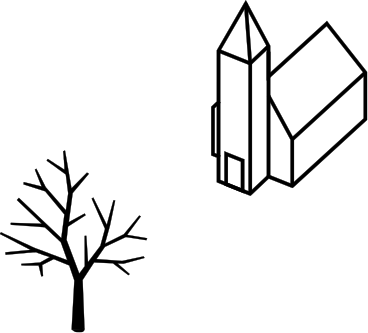
\includegraphics[width=.5\textwidth]{figure-ground-array}
\caption{Figure-ground array}
\label{fig:figure}
\end{figure}
 
\subsection{Quotations}
``Enclose quotations up to three lines with double quotation marks.  Note that a fullstop appears before the closing quotation mark.'' 
\begin{quote}
  Use block quotes only for quotations exceeding three lines.  Quotation marks are not needed in this case.  Indicate any omissions with ``\ldots'' (\verb|\ldots|), e.g.\ ``\citeauthor*{GuilfoyleHungTravis92} \citeyearpar{GuilfoyleHungTravis92} claim \ldots\ that their names should not be omitted.''
\end{quote}

\currentpdfbookmark{Abbreviations}{Abbreviations}
\section*{Abbreviations} 
List all the abbreviations used in your paper, including those in the Leipzig Glossing Rules list, here.  You may typeset the list as follows.  Without a specific font shape option, \verb|\abbrev| will typeset its first argument in \textsc{small caps}.

\begin{lstlisting}
\begin{abbreviations}
  \abbrev{1}{first person}
  \abbrev{2}{second person}
  \abbrev{3}{third person}
  \abbrev{clf}{classifier}
  \abbrev{DP}{determiner phrase}
  \abbrev{excl}{exclusive}
  ...
  \abbrev[\textrm]{Spec}{specifier}
  \abbrev[\textit]{t}{trace}
\end{abbreviations}
\end{lstlisting}

\begin{abbreviations}
  \abbrev{1}{first person}
  \abbrev{2}{second person}
  \abbrev{3}{third person}
%  \abbrev{A}{agent-like argument of canonical transitive verb}
%  \abbrev{abl}{ablative}
%  \abbrev{abs}{absolutive}
%  \abbrev{acc}{accusative}
%  \abbrev{adj}{adjective}
%  \abbrev{adv}{adverb(ial)}
%  \abbrev{agr}{agreement}
%  \abbrev{all}{allative}
%  \abbrev{antip}{antipassive}
%  \abbrev{appl}{applicative}
%  \abbrev{art}{article}
%  \abbrev{aux}{auxiliary}
%  \abbrev{ben}{benefactive}
%  \abbrev{caus}{causative}
  \abbrev{clf}{classifier}
%  \abbrev{com}{comitative}
%  \abbrev{comp}{complementizer}
%  \abbrev{compl}{completive}
%  \abbrev{cond}{conditional}
%  \abbrev{cop}{copula}
%  \abbrev{cvb}{converb}
%  \abbrev{dat}{dative}
%  \abbrev{decl}{declarative}
%  \abbrev{def}{definite}
%  \abbrev{dem}{demonstrative}
%  \abbrev{det}{determiner}
%  \abbrev{dist}{distal}
%  \abbrev{distr}{distributive}
  \abbrev{DP}{determiner phrase}
%  \abbrev{du}{dual}
%  \abbrev{dur}{durative}
%  \abbrev{erg}{ergative}
  \abbrev{excl}{exclusive}
%  \abbrev{f}{feminine}
%  \abbrev{foc}{focus}
%  \abbrev{fut}{future}
%  \abbrev{gen}{genitive}
%  \abbrev{imp}{imperative}
  \abbrev{incl}{inclusive}
%  \abbrev{ind}{indicative}
%  \abbrev{indf}{indefinite}
%  \abbrev{inf}{infinitive}
%  \abbrev{ins}{instrumental}
%  \abbrev{intr}{intransitive}
%  \abbrev{ipfv}{imperfective}
%  \abbrev{irr}{irrealis}
%  \abbrev{loc}{locative}
%  \abbrev{m}{masculine}
%  \abbrev{n}{neuter}
%  \abbrev{n-}{non- (e.g.\ \textsc{nsg} nonsingular, \textsc{npst} nonpast)}
%  \abbrev{neg}{negation, negative}
%  \abbrev{nmlz}{nominalizer/nominalization}
%  \abbrev{nom}{nominative}
  \abbrev{NP}{noun phrase}
%  \abbrev{obj}{object}
%  \abbrev{obl}{oblique}
  \abbrev{P}{preposition}
%  \abbrev{P}{patient-like argument of canonical transitive verb}
  \abbrev{part}{particle}
  \abbrev{pass}{passive}
%  \abbrev{pfv}{perfective}
  \abbrev{pl}{plural}
%  \abbrev{poss}{possessive}
  \abbrev{PP}{preposition phrase}
%  \abbrev{pred}{predicative}
  \abbrev{prf}{perfect}
%  \abbrev{prs}{present}
%  \abbrev{prog}{progressive}
%  \abbrev{proh}{prohibitive}
%  \abbrev{prox}{proximal/proximate}
%  \abbrev{pst}{past}
%  \abbrev{ptcp}{participle}
%  \abbrev{purp}{purposive}
%  \abbrev{q}{question particle}
  \abbrev{q}{question marker}
%  \abbrev{quot}{quotative}
%  \abbrev{recp}{reciprocal}
%  \abbrev{refl}{reflexive}
%  \abbrev{rel}{relative}
  \abbrev{rel}{relativizer}
%  \abbrev{res}{resultative}
%  \abbrev{S}{single argument of canonical intransitive verb}
%  \abbrev{sbj}{subject}
%  \abbrev{sbjv}{subjunctive}
  \abbrev{sg}{singular}
  \abbrev[\textrm]{Spec}{specifier}
  \abbrev[\textit]{t}{trace}
%  \abbrev{top}{topic}
%  \abbrev{tr}{transitive}
%  \abbrev{voc}{vocative}
\end{abbreviations}

\currentpdfbookmark{References}{References}
% \bibliography{references}
\begin{thebibliography}{5}
\providecommand{\natexlab}[1]{#1}

\bibitem[{Alwi et~al.(1998)Alwi, Dardjowidjojo, Lapoliwa \&
  Moeliono}]{Alwi_dkk98}
Alwi, Hasan, Soenjono Dardjowidjojo, Hans Lapoliwa \& Anton~M. Moeliono. 1998.
\newblock \emph{Tata bahasa baku bahasa {I}ndonesia}\textsf{, edisi ketiga}.
\newblock Jakarta: Balai Pustaka.
\newblock \par \textsf{The edition information needs to be edited manually.}

\bibitem[{Arka \& Manning(1998)}]{ArkaManning98}
Arka, I~Wayan \& Christopher~D. Manning. 1998.
\newblock Voice and grammatical relations in {I}ndonesian: A new perspective.
\newblock In Mirriam Butt \& Tracy~Holloway King (eds.), \emph{Proceedings of
  the {LFG98} conference}. Stanford, CA: CSLI Publications.

\bibitem[{Asmah \& Rama(1968)}]{AsmahRama68}
  \textsf{Asmah Haji~Omar} \& Subbiah Rama. 1968.
\newblock \emph{An introduction to {M}alay grammar}.
\newblock Kuala Lumpur: Dewan Bahasa dan Pustaka.
\newblock \par \textsf{Muslim names can be written as either `given\_name father's\_name' or `father's\_name, given\_name'.  Use the former style for Malaysian, Singaporean and Brunei authors.}

\bibitem[{Guilfoyle et~al.(1992)Guilfoyle, Hung \&
  Travis}]{GuilfoyleHungTravis92}
Guilfoyle, Eithene, Henrietta Hung \& Lisa Travis. 1992.
\newblock Spec of {IP} and {S}pec of {VP}: Two subjects in {A}ustronesian
  languages.
\newblock \emph{Natural Language and Linguistic Theory} 10. 375--414.

\bibitem[{Shiohara(2010)}]{Shiohara10}
Shiohara, Asako. 2010.
\newblock Sunbawago no genkou nikakawaru settouji \textit{N-} to \textit{bar-}
 \textsf{[The two valence-decreasing prefixes \textit{N-} and \textit{bar-} of
 {S}umbawa]}.
\newblock \emph{Ajia-Afurika no Gengo to Gengogaku} 4. 61--84.
\newblock \par \textsf{Provide translation for titles in languages other than English and Standard Malay/Indonesian.}

\end{thebibliography}
\end{document}
